% !TEX program = pdflatex
\documentclass[11pt]{article}
\setlength{\textwidth}{6.5in}
\setlength{\oddsidemargin}{0pt}
\setlength{\evensidemargin}{0pt}
\setlength{\textheight}{9in}
\setlength{\topmargin}{0pt}
\addtolength{\topmargin}{-\headheight}
\addtolength{\topmargin}{-\headsep}
\ifdefined\pdfpagewidth \pdfpagewidth=8.5in \pdfpageheight=11in \fi
\ifdefined\pagewidth \pagewidth=8.5in \pageheight=11in \fi
\usepackage{amsmath,amssymb}
\usepackage{array}
\usepackage{booktabs}
\usepackage[tableposition=top]{caption}
\usepackage{longtable}
\usepackage{enumitem}
\usepackage{tikz}
\usepackage{pgfplots}
\pgfplotsset{compat=1.18}
\emergencystretch=3em

% ---- notation ---------------------------------------------------------------
\newcommand{\um}{\,$\mu$m}
\newcommand{\kms}{km\,s$^{-1}$}
\newcommand{\flux}{erg\,cm$^{-2}$\,s$^{-1}$}
\newcommand{\mA}{m\AA}
\newcommand{\sci}[2]{#1\times10^{#2}}
\newcommand{\ion}[2]{#1\,\textsc{#2}}
\newcommand{\nuc}[2]{$^{#1}$#2}
\newcommand{\lxl}{$L_X/L_\mathrm{bol}$}

% ---- front matter -----------------------------------------------------------
\title{HD 31435: a Five Per Cent Polarisation\\ Assigned to an Unreddened Sun-like Star at 100\,pc}
\author{Charles C. Norton}
\date{}

\begin{document}
\maketitle

\begin{abstract}
Starlight from a quiet dwarf in front of the interstellar dust is polarised at parts
per million, and a structure that reflects part of a star's light polarises it, so a
nearby, unreddened dwarf polarised at the per cent level has no ordinary explanation at
the star. We test the $28704$ stars of the Panopoulou et al.\ compilation of optical
polarimetry that have five or more neighbours within $3^\circ$ and $20$ per cent in
distance for a Stokes vector their neighbours do not share. Four dwarfs within
$200$\,pc are discordant at $5\sigma$; three are a cloud's own dust, a binary in a
crowded field and an interstellar sightline that Gaia and Planck recognise. The fourth,
HD~31435, an F9/G0 dwarf at $100$\,pc, is listed at $5.48\pm0.15$ per cent and
$47^\circ$ in Johnson $V$ from one measurement of 1977 November, where the eleven
stars of its field within $130$\,pc read $0.27$ per cent or less. Nothing at the star
accounts for it: Gaia gives no reddening, the star is single and steady in Gaia's
astrometry and velocities and in TESS, K2, Hipparcos and the Harvard plates, and WISE
sees its photosphere to $22$\um. A reflector would have to return several per cent of
its light, grey to $0.3$ per cent from $400$ to $700$\,nm in its Gaia XP spectrum
against $40$ twins; Gaia's image statistics and Pan-STARRS leave no room for it from
$10$ to $1300$\,au, and within $10$\,au only one that absorbs nothing and holds still
escapes WISE and the light curves. The angle is the interstellar field's behind the
Taurus clouds: the $40$ stars of the field beyond $160$\,pc read a median $48^\circ$,
and Planck's $353$\,GHz polarisation at the position predicts $49$ to $54^\circ$. The
amount is what background stars there reach on efficient sightlines, three of those
$40$ at $5.5$ per cent or more. HD~283904, a reddened A2 star of the same brightness
behind the cloud, lies $5'$ west at the same declination to $27''$, $23$\,s of right
ascension away. The measurement is that of a star behind the cloud, most likely
HD~283904 through a slipped setting, and one polarimetric measurement of the two stars
decides.
\end{abstract}

% =============================================================================
\section{Introduction}\label{sec:intro}
% =============================================================================

The light of a nearby, inactive dwarf is polarised at a few parts per million: the
brightest southern stars within the Local Bubble, measured at that level, carry
interstellar polarisations of tens of ppm and intrinsic ones too small to
separate~\cite{Cotton2016}. Interstellar polarisation grows with the dust in front of a
star and is bounded by it, $p\le9\,E(B-V)$ per cent in the visible~\cite{Serkowski1975},
so a star in front of the dust carries almost none. Reflection polarises: sunlight
scattered from a planet's atmosphere or reflected from a flat surface is polarised by
an amount set by the scattering angle and the material, and a structure that returns
part of a star's light toward Earth would add that polarised light to the star's. A
dwarf in front of the dust whose polarisation reaches the per cent level therefore has
no explanation at the star that the archives would not show, and one that a reflector
would give.

Optical polarimetry of stars has been gathered from many programmes into
compilations~\cite{Heiles2000,Panopoulou2025}, and with Gaia distances each star can be
set against its neighbours on the sky at the same distance, which share its
interstellar column. This note reports that test and the one star it leaves, HD~31435,
and reads its measurement against every archive that bears on it.

\subsection{Contributions}
\begin{enumerate}[leftmargin=*,itemsep=1pt]
\item A test of $28704$ stars with optical polarimetry and Gaia distances against their
neighbours' Stokes vectors, with the measurements reassigned among neighbours as the
null.
\item For HD~31435, the one discordant dwarf left, the constraints of Gaia, WISE, TESS,
K2, Hipparcos, DASCH, Gaia XP and Pan-STARRS on any source of polarised light at the
star, and the reading of its measurement against the field, Planck's dust polarisation
and the star of the same brightness beside it.
\end{enumerate}

% =============================================================================
\section{The screen}\label{sec:screen}
% =============================================================================

The compilation of Panopoulou et al.~\cite{Panopoulou2025} holds $55742$ measurements
from $81$ publications, with Gaia EDR3 identifiers and distances; $37210$ stars carry
Stokes $q$ and $u$. Of these, $29442$ are unflagged and have five or more neighbours
within $3^\circ$ and within $20$ per cent of their distance, and $28704$ of them can be
judged against neighbours from their own catalogue, which removes the zero-point
differences between programmes. A star's residual is its Stokes vector less the
neighbours' mean, divided by its own error and the neighbours' scatter in quadrature.
The same statistic with each field's measurements reassigned among its stars is the
null. Residuals above $3\sigma$ occur in $8.3$ per cent of the stars against $7.4$ per
cent in the null, and above $5\sigma$ in $1.2$ against $0.9$ per cent, so discordance
at that level is mostly the scatter of real sightlines.

We keep dwarfs within $200$\,pc, where the interstellar column is small, whose residual
reaches $5\sigma$, exceeds $0.1$ per cent and five times the field's scatter, and
departs from the field in angle or lies in an unpolarised field. Four remain. HD~142832,
an F3 dwarf at $158$\,pc, was measured in the survey of the Lupus~1 cloud of Alves and
Franco~\cite{AlvesFranco2006} and lies at the cloud's distance, where its dust
polarises it and not its nearer neighbours. Dachs SMC~2-61, a G5 dwarf at $134$\,pc
with a renormalised unit weight error (RUWE) of $8.9$ and an X-ray counterpart, was
measured in a crowded field toward the Small Magellanic Cloud and is a binary or a
blend. HD~127769, an A7 dwarf at $187$\,pc, read $1.3$ per cent at $43^\circ$ in the
compilation of Heiles~\cite{Heiles2000} against its field's $0.4$ per cent at $87^\circ$;
Gaia gives it an extinction $A_G=0.32$\,mag where its nearer neighbours have none, and
Planck's $353$\,GHz dust emission at its position is polarised at $18$ per cent with a
field that predicts $52^\circ$ and $1.9$ per cent for starlight behind the full column,
so its measurement sits on that sightline. The fourth is HD~31435.

% =============================================================================
\section{HD 31435}\label{sec:hd}
% =============================================================================

\subsection{The measurement}

HD~31435 (Gaia DR3 154235505416809344) is an F9/G0 dwarf at $100.1$\,pc with
$G=8.90$, $G_\mathrm{BP}-G_\mathrm{RP}=0.73$ and $M_G=3.85$, at the main-sequence
turnoff of an $8$ to $9$\,Gyr population. The compilation gives
$q=-0.38\pm0.15$ and $u=+5.47\pm0.15$ per cent, $p=5.48\pm0.15$ per cent at position
angle $47.0\pm0.8^\circ$ in Johnson $V$, from a Minipol~\cite{Frecker1976} measurement on
JD~2443471.5, 1977 November 22, published by name in Table~2 of Moneti et
al.~\cite{Moneti1984}, whose survey measured field stars toward the Taurus dark clouds.
Against the mean of its neighbours, $0.04$ per cent at $77^\circ$, the residual is
$5.46$ per cent at $46.8^\circ$, $28.9\sigma$. No other polarimetry of the star is found
among the $135$ VizieR catalogues with entries at its position, and the other $93$ stars
of that programme read below $0.4$ per cent within $130$\,pc and rise with reddening
beyond it.

Figure~\ref{fig:field} shows the field. The compilation holds $58$ stars within $3^\circ$
of HD~31435: the $11$ within $130$\,pc read $0.27$ per cent or less, and the $40$
beyond $160$\,pc, behind the Taurus clouds, read a median of $3.2$ per cent, with a
$90$th percentile of $4.9$ per cent and three of the $40$ at $5.5$ per cent or more, at
a median angle of $48^\circ$ and a $16$th to $84$th percentile range of $35$ to
$61^\circ$. HD~31435 lies at the distance of the unpolarised stars with the
polarisation of the background ones.

\begin{figure}[tp]
\centering
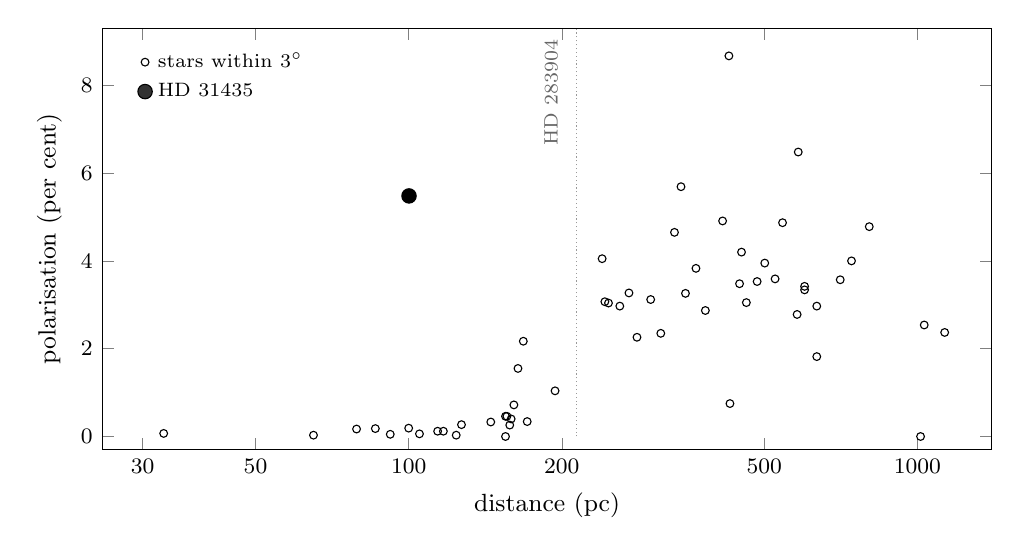
\begin{tikzpicture}
\begin{semilogxaxis}[width=0.78\textwidth,height=0.42\textwidth,xmin=25,xmax=1400,ymin=-0.3,ymax=9.3,
  xlabel={distance (pc)},ylabel={polarisation (per cent)},tick label style={font=\footnotesize},label style={font=\small},
  xtick={30,50,100,200,500,1000},xticklabels={$30$,$50$,$100$,$200$,$500$,$1000$},
  legend style={font=\scriptsize,at={(0.03,0.97)},anchor=north west,draw=none,fill=white,fill opacity=0.8,text opacity=1},legend cell align=left]
\addplot[only marks,mark=o,mark size=1.4pt,black] coordinates {(33,0.070) (65,0.030) (79,0.170) (86,0.180) (92,0.050) (100,0.190) (105,0.060) (114,0.120) (117,0.120) (124,0.030) (127,0.270) (145,0.330) (155,0.000) (155,0.460) (156,0.460) (158,0.260) (159,0.400) (161,0.720) (164,1.550) (168,2.170) (171,0.340) (194,1.040) (240,4.050) (243,3.070) (247,3.040) (260,2.970) (271,3.270) (281,2.260) (299,3.120) (313,2.350) (333,4.650) (343,5.690) (350,3.260) (367,3.830) (383,2.870) (414,4.910) (426,8.670) (428,0.750) (447,3.480) (451,4.200) (461,3.050) (484,3.530) (501,3.950) (525,3.590) (543,4.870) (580,2.780) (583,6.480) (600,3.340) (600,3.420) (634,2.970) (634,1.820) (705,3.570) (742,4.000) (804,4.780) (1014,0.000) (1031,2.540) (1131,2.370)};
\addlegendentry{stars within $3^\circ$}
\addplot[only marks,mark=*,mark size=2.6pt,black] coordinates {(100.15,5.48)};
\addlegendentry{HD 31435}
\addplot[black!40,densely dotted,forget plot] coordinates {(214,0) (214,9.3)};
\node[font=\scriptsize,text=black!60,anchor=south west,rotate=90] at (axis cs:205,6.4) {HD 283904};
\end{semilogxaxis}
\end{tikzpicture}
\caption{Optical polarisation against Gaia distance for the $58$ stars of the
compilation within $3^\circ$ of HD~31435, with HD~31435 filled. The dotted line marks
the distance of HD~283904, which has no measurement.}
\label{fig:field}
\end{figure}

\subsection{The star}

Nothing at the star gives per cent polarisation. Interstellar polarisation of
$5.48$ per cent needs $E(B-V)\ge0.6$\,mag~\cite{Serkowski1975}; Gaia's astrophysical
parameters give $E(G_\mathrm{BP}-G_\mathrm{RP})=0.00$, and the star's $B-V$ of $0.565$
lies $0.015$\,mag blueward of the intrinsic colour of its type. The WISE
photometry~\cite{Wright2010} follows the photosphere from $3.4$ to $22$\um, with no warm
dust. Its astrometry carries no companion: RUWE $0.99$, no multiple image peaks, and a
Hipparcos--Gaia proper-motion anomaly~\cite{Kervella2022} of $20\pm32$\,m\,s$^{-1}$. Gaia's
radial velocity, from $17$ transits over $920$ days, varies by less than
$1$\,km\,s$^{-1}$. TESS~\cite{Ricker2015},
K2~\cite{Howell2014} and Hipparcos~\cite{Perryman1997} photometry is flat to $0.03$ per
cent, and the Harvard plates~\cite{Grindlay2009} show no dimming around 1977 against
matched stars on the same plates. The star is an old, single, quiet dwarf in front of the
dust, whose intrinsic polarisation would be of order ten ppm.

\subsection{A reflector}

Light reflected by a structure near the star and seen together with it is polarised by
$p\approx fP_r$, with $f$ the fraction of the star's light returned toward Earth and
$P_r$ the polarisation of the reflected light, so $5.48$ per cent needs $f\ge0.055$ even
if every reflected photon is polarised. Specular reflection from metals polarises
weakly away from grazing incidence: by the Fresnel relations aluminium gives $3$ to $14$
per cent at incidence angles of $45$ to $80^\circ$ and silver less than $2$ per cent, so
a metal mirror needs $f$ of order one, and a dielectric reaches $98$ per cent at
Brewster's angle while reflecting $9$ per cent of what falls on it, so it must
intercept more than half of the star's light. Only a reflector that sends back one
polarisation and passes or absorbs the other, as a conducting grid does, gives
$5.5$ per cent with $f\approx0.06$.

The reflected light carries the reflector's colour. Against the median of $40$ Gaia XP
spectra~\cite{DeAngeli2023} of unreddened twins matched in temperature, gravity and
metallicity, HD~31435's spectrum agrees to $0.3$ per cent from $400$ to $700$\,nm
($0.9998\pm0.0013$, $0.9970\pm0.0005$ and $1.0013\pm0.0011$ in the three $100$\,nm
bands) and lies $0.35$ and $0.66$ per cent high at $700$ to $800$ and $800$ to $900$\,nm,
within the twins' own spread of $0.7$ to $1.0$ per cent there; its slope,
$+0.0014$ per $100$\,nm, lies inside the twins' $-0.005$ to $+0.006$. Aluminium's
reflectance dips by about six per cent near $830$\,nm, so a tenth of the light
reflected from aluminium would take $0.6$ per cent out of the $800$ to $900$\,nm band,
where HD~31435 lies above its twins rather than below them. The spectrum is that of a
star with nothing coloured added to it, and leaves a grey reflector.

The reflector must also lie where no archive sees it. A structure within about
$10$\,au that absorbs as little as a per cent of what it intercepts would radiate above
the photosphere at $22$\um, which WISE excludes; one that absorbs nothing is not
excluded there, and TESS, K2 and Hipparcos, flat to $0.03$ per cent over years, exclude
one whose reflected light changes along an orbit, so what is left inside $10$\,au is a
perfect reflector that holds still. Gaia's image parameters, with RUWE $0.99$ and no
second peak, exclude a resolved source of a few per cent of the star's light at $0.1$ to
$2''$, $10$ to $200$\,au. Pan-STARRS~\cite{Chambers2016} images in $g$, $r$, $i$, $z$
and $y$, with each radial profile normalised at $13$ to $25''$ against three stars of
like brightness in the same frames, show no excess light at $2$ to $13''$ in any filter,
so no extended reflector lies at $200$ to $1300$\,au.

\subsection{The sightline}

The measured angle is the field's. Planck's $353$\,GHz maps~\cite{Planck2020}, read at
HD~31435's position on the HEALPix grid~\cite{Gorski2005}, give dust emission polarised
at $6$ to $8$ per cent with a polarised intensity of $0.12$ to $0.15$\,MJy\,sr$^{-1}$
within $5$ to $20'$; turned through $90^\circ$ and into the equatorial frame, the field
predicts $49$ to $54^\circ$ for starlight behind the column, against the measured
$47^\circ$ and the background stars' median of $48^\circ$. The ratio of polarised
submillimetre intensity to optical polarisation, $5.4$\,MJy\,sr$^{-1}$~\cite{Planck2015},
predicts $2.3$ to $2.8$ per cent for a star behind the whole column, half the measured
value; sightlines scatter about that ratio, and three of the field's $40$ background
stars reach $5.5$ per cent or more.

The star of the same brightness beside HD~31435 is behind the cloud. HD~283904, an A2
star at $214$\,pc with $A_G=1.3$\,mag and the $1.527$\um\ diffuse interstellar
band~\cite{Zasowski2015} in its APOGEE spectrum~\cite{Majewski2017}, lies $5'$ west of
HD~31435, at the same declination to $27''$ and $23$\,s of right ascension away, and has
never been measured. A setting that slipped by $23$\,s of hour angle would have placed it
in the aperture in place of HD~31435, and its polarisation would be the field's: the
angle exactly, and the amount on an efficient sightline.

% =============================================================================
\section{Related work}\label{sec:related}
% =============================================================================

Polarimetry of nearby stars at parts per million~\cite{Cotton2016} measures the
interstellar polarisation inside the Local Bubble and bounds the intrinsic polarisation
of dwarfs, and the compilations of optical
polarimetry~\cite{Heiles2000,Panopoulou2025}, joined to Gaia distances, are used to map
the interstellar field and the dust in three dimensions. Planck's comparison of
submillimetre and optical polarisation~\cite{Planck2015} gives the ratio used here to
predict a star's polarisation from the dust emission at its position. We find no earlier
use of these compilations to look for stars whose polarisation their neighbours do not
share, nor any discussion of HD~31435's measurement.

% =============================================================================
\section{Conclusion}\label{sec:conclusion}
% =============================================================================

Among $28704$ stars with optical polarimetry, one dwarf within $200$\,pc carries a
polarisation that neither its neighbours nor anything at the star accounts for: HD~31435,
listed at $5.48$ per cent from a single measurement of 1977. A reflector that made it
would have to return at least six per cent of the star's light, be grey across the
visible to a third of a per cent and polarise like a conducting grid, either lie within
$10$\,au, absorb nothing and hold still or lie beyond $1300$\,au, and be aligned by
chance with the Galaxy's field behind the Taurus clouds. The measurement has instead
every property of a star behind those clouds, and a star of the same brightness behind
them sits $23$\,s of right ascension away. The measurement most likely belongs to
HD~283904.

Measuring both stars in one night with any polarimeter of $0.1$ per cent precision
decides between the two readings, and measuring HD~31435 at parts per million would
bound what a reflector could hide at the level the Local Bubble's stars set.

\section*{Acknowledgements}

This work uses the compilation of optical starlight polarisation of Panopoulou et al.\
and the agglomeration of Heiles through VizieR at CDS, Strasbourg; data from the
European Space Agency mission Gaia, processed by the Gaia Data Processing and Analysis
Consortium (DPAC), funded by national institutions, in particular those participating
in the Gaia Multilateral Agreement; Planck maps from the NASA/IPAC Infrared Science
Archive; WISE, TESS and K2 data from IRSA and MAST; the Pan-STARRS1 image cutout service;
SDSS-IV's APOGEE; the DASCH project's digitised Harvard plates; and the software astropy,
astropy-healpix, NumPy and SciPy.

\begin{thebibliography}{99}\small\raggedright
\setlength{\itemsep}{1pt}

\bibitem{Cotton2016}
D.~V. Cotton, J.~Bailey, L.~Kedziora-Chudczer, et al., The linear polarization of
Southern bright stars measured at the parts-per-million level, \emph{Mon. Not. R. Astron.
Soc.} \textbf{455}, 1607 (2016).

\bibitem{Serkowski1975}
K.~Serkowski, D.~S. Mathewson and V.~L. Ford, Wavelength dependence of interstellar
polarization and ratio of total to selective extinction, \emph{Astrophys. J.}
\textbf{196}, 261 (1975).

\bibitem{Heiles2000}
C.~Heiles, 9286 stars: an agglomeration of stellar polarization catalogs, \emph{Astron.
J.} \textbf{119}, 923 (2000).

\bibitem{Panopoulou2025}
G.~V. Panopoulou, L.~Markopoulioti, F.~Bouzelou, et al., A compilation of optical
starlight polarization catalogs, \emph{Astrophys. J. Suppl.} \textbf{276}, 15 (2025).

\bibitem{AlvesFranco2006}
F.~O. Alves and G.~A.~P. Franco, The magnetic field in the Lupus I molecular cloud,
\emph{Mon. Not. R. Astron. Soc.} \textbf{366}, 238 (2006).

\bibitem{Frecker1976}
J.~E. Frecker and K.~Serkowski, Linear polarimeter with rapid modulation, achromatic in
the $0.3$--$1.1$\,$\mu$m range, \emph{Appl. Opt.} \textbf{15}, 605 (1976).

\bibitem{Moneti1984}
A.~Moneti, J.~L. Pipher, H.~L. Helfer, R.~S. McMillan and M.~L. Perry, Magnetic field
structure in the Taurus dark cloud, \emph{Astrophys. J.} \textbf{282}, 508 (1984).

\bibitem{Wright2010}
E.~L. Wright, P.~R.~M. Eisenhardt, A.~K. Mainzer, et al., The Wide-field Infrared Survey
Explorer (WISE): mission description and initial on-orbit performance, \emph{Astron. J.}
\textbf{140}, 1868 (2010).

\bibitem{Kervella2022}
P.~Kervella, F.~Arenou and F.~Th\'evenin, Stellar and substellar companions from Gaia
EDR3: proper-motion anomaly and resolved common proper-motion pairs, \emph{Astron.
Astrophys.} \textbf{657}, A7 (2022).

\bibitem{Ricker2015}
G.~R. Ricker, J.~N. Winn, R.~Vanderspek, et al., Transiting Exoplanet Survey Satellite,
\emph{J. Astron. Telesc. Instrum. Syst.} \textbf{1}, 014003 (2015).

\bibitem{Howell2014}
S.~B. Howell, C.~Sobeck, M.~Haas, et al., The K2 mission: characterization and early
results, \emph{Publ. Astron. Soc. Pac.} \textbf{126}, 398 (2014).

\bibitem{Perryman1997}
M.~A.~C. Perryman, L.~Lindegren, J.~Kovalevsky, et al., The Hipparcos catalogue,
\emph{Astron. Astrophys.} \textbf{323}, L49 (1997).

\bibitem{Grindlay2009}
J.~Grindlay, S.~Tang, R.~Simcoe, et al., DASCH to measure (and preserve) the Harvard
plates: opening the $\sim$100-year time domain astronomy window, in \emph{Preserving
Astronomy's Photographic Legacy}, ASP Conf. Ser. \textbf{410}, 101 (2009).

\bibitem{DeAngeli2023}
F.~De~Angeli, M.~Weiler, P.~Montegriffo, et al., Gaia Data Release 3: processing and
validation of BP/RP low-resolution spectral data, \emph{Astron. Astrophys.}
\textbf{674}, A2 (2023).

\bibitem{Chambers2016}
K.~C. Chambers, E.~A. Magnier, N.~Metcalfe, et al., The Pan-STARRS1 surveys,
arXiv:1612.05560 (2016).

\bibitem{Planck2020}
Planck Collaboration, Planck 2018 results. III. High Frequency Instrument data
processing and frequency maps, \emph{Astron. Astrophys.} \textbf{641}, A3 (2020).

\bibitem{Gorski2005}
K.~M. G\'orski, E.~Hivon, A.~J. Banday, et al., HEALPix: a framework for
high-resolution discretization and fast analysis of data distributed on the sphere,
\emph{Astrophys. J.} \textbf{622}, 759 (2005).

\bibitem{Planck2015}
Planck Collaboration, Planck intermediate results. XXI. Comparison of polarized thermal
emission from Galactic dust at 353 GHz with interstellar polarization in the visible,
\emph{Astron. Astrophys.} \textbf{576}, A106 (2015).

\bibitem{Zasowski2015}
G.~Zasowski, B.~M\'enard, D.~Bizyaev, et al., Mapping the interstellar medium with
near-infrared diffuse interstellar bands, \emph{Astrophys. J.} \textbf{798}, 35 (2015).

\bibitem{Majewski2017}
S.~R. Majewski, R.~P. Schiavon, P.~M. Frinchaboy, et al., The Apache Point Observatory
Galactic Evolution Experiment (APOGEE), \emph{Astron. J.} \textbf{154}, 94 (2017).

\end{thebibliography}

\end{document}
